% !TEX root = ../paper.tex
\section{Results and Examples}

\subsection{Forge as a Lean DSL}
One of the crucial benefits of working with Lean 4 as a metaprogramming language and a target for our translation is the rich support for DSL implementation and integration. Lean and its accompanying Language Server Protocol (LSP)\footnote{This is the language server that processes Lean code and communicates with the code editor or integrated development environment. In this case, we use VS Code.} are designed to have highly flexible and extensiblie user interfaces that expose useful APIs for implementers of DSLs and custom UI to utilize \cite{moura2021lean, nawrocki2023extensible}. Furthermore, Lean's extensible syntax and macro system are simple yet remarkably powerful \cite{ullrich2022beyond, metaprogramming}. 

It is as such that we justify framing our implementation of Forge in Lean as an honest-to-goodness domain-specific language (DSL). We do not treat user-experience of our tool as an afterthought, nor do we skimp over ensuring that LForge has a set of developer aids just as capable as those found in Forge or Lean themselves. As mentioned in \cref{sec:design-summary}, the fact that we are able to interact with Lean's own implementation means that many of Lean's `IDE-like' features are exposed to us and available for us to use in the Forge DSL without much overhead. 

The following are some (non-exhaustive) examples of the user experience and interface of Forge within Lean. 

\subsubsection{Syntax Highlighting}

Superficially, by virtue of defining our syntax as Lean objects and isolating our keywords (we piggyback off Lean's lexer), we get syntax highlighting of Forge code `for free', on par with Forge's native solutions. In \cref{fig:sc-highlighting-hover}, the syntax of a Forge specification is highlighted. 

\subsubsection{Types on Hover}

Lean exposes an \texttt{addTermInfo'} method that allows us to attach declared names to pieces of syntax (nodes in Lean's concrete syntax tree), including custom syntax like ours for Forge. As such, we can annotate relevant pieces of syntax within our Forge specification to reflect names and types that are within scope. When the user hovers their mouse over a piece of syntax corresponding to a Forge expression, a hovering tooltip will display with the type of the expression. In \cref{fig:sc-highlighting-hover}, the tooltip shows the type of a Forge predicate defined earlier in the file. 

\begin{figure}
  \centering
  \fbox{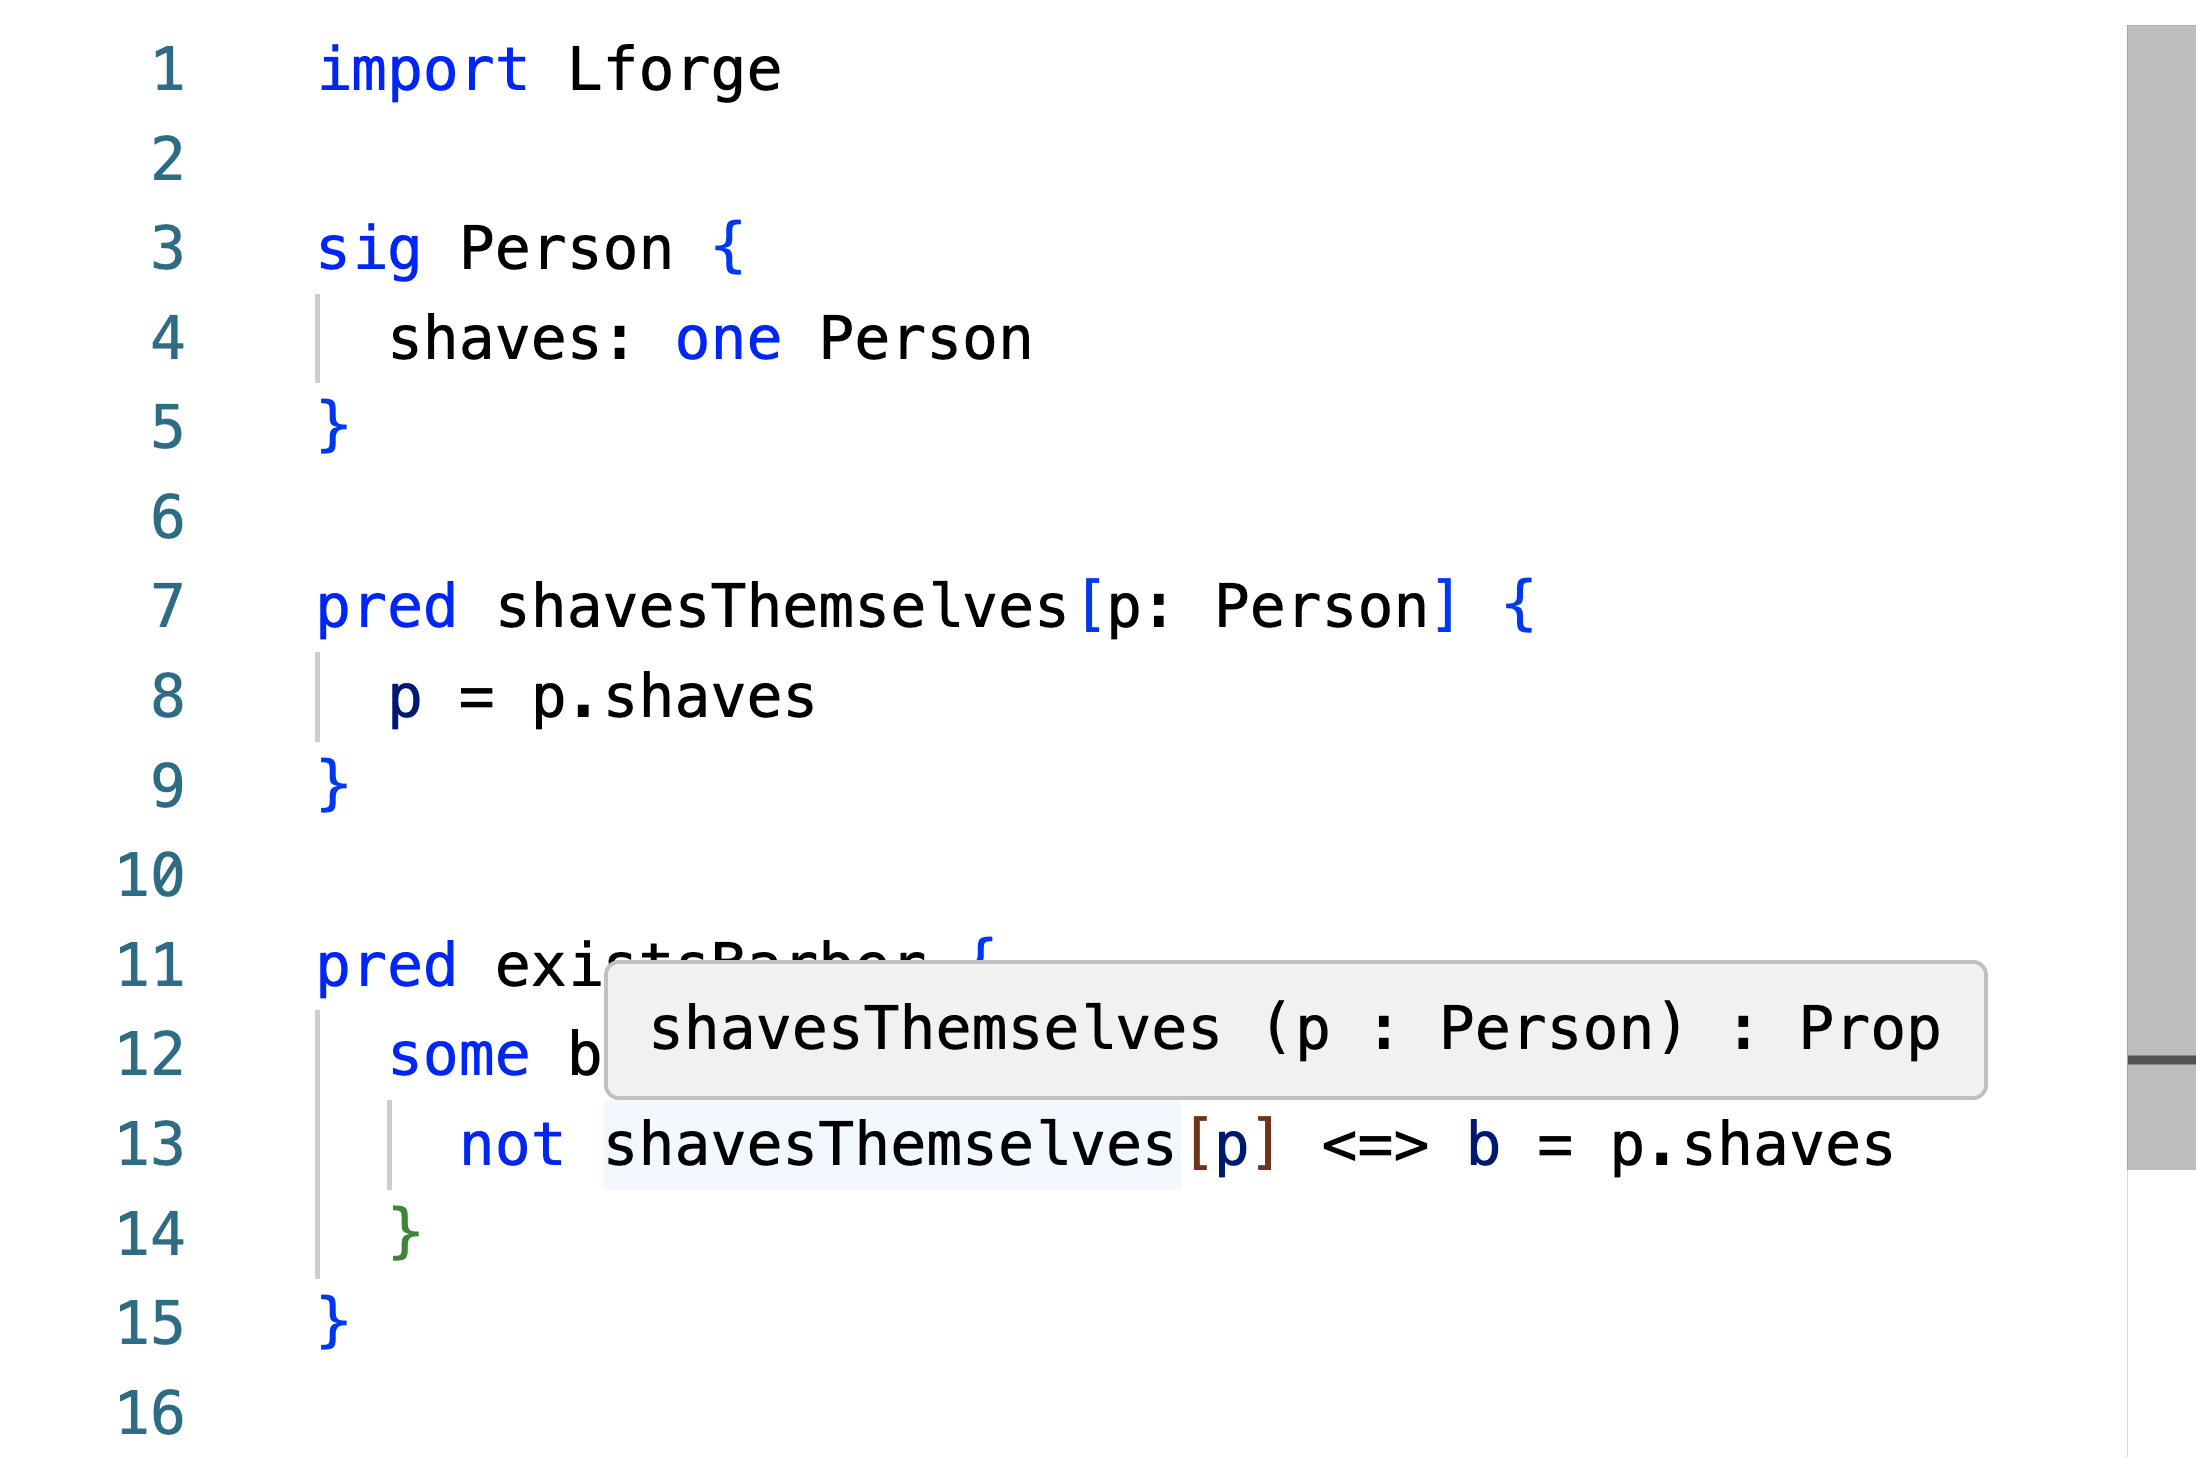
\includegraphics[width=0.5\textwidth,trim={0 0 2cm 0},clip]{images/screenshots/hover-tooltip.png}}
  \caption{Tooltips containing type information are available on hover. Forge syntax is automatically highlighted without any extra work.}
  \label{fig:sc-highlighting-hover}
\end{figure}

\begin{figure}
  \begin{center}
    \fbox{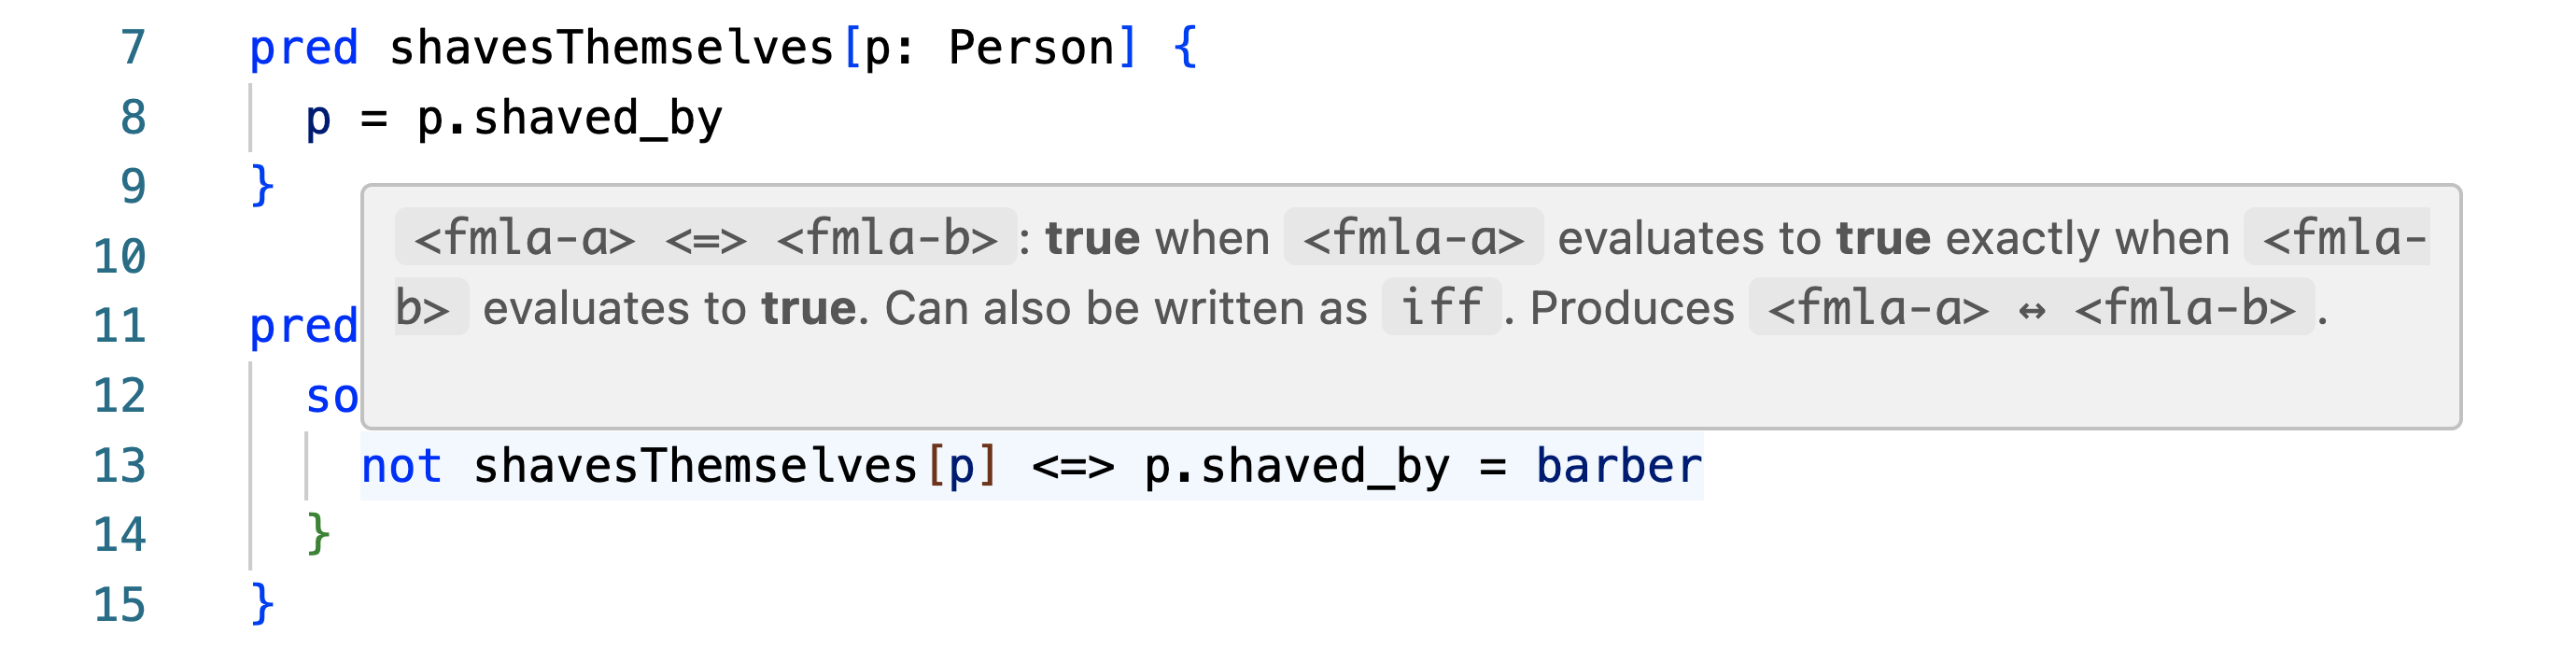
\includegraphics[width=0.6\textwidth,trim={0 0 0 0},clip]{images/screenshots/documentation.png}}
  \end{center}
  \begin{center}
    \centering\fbox{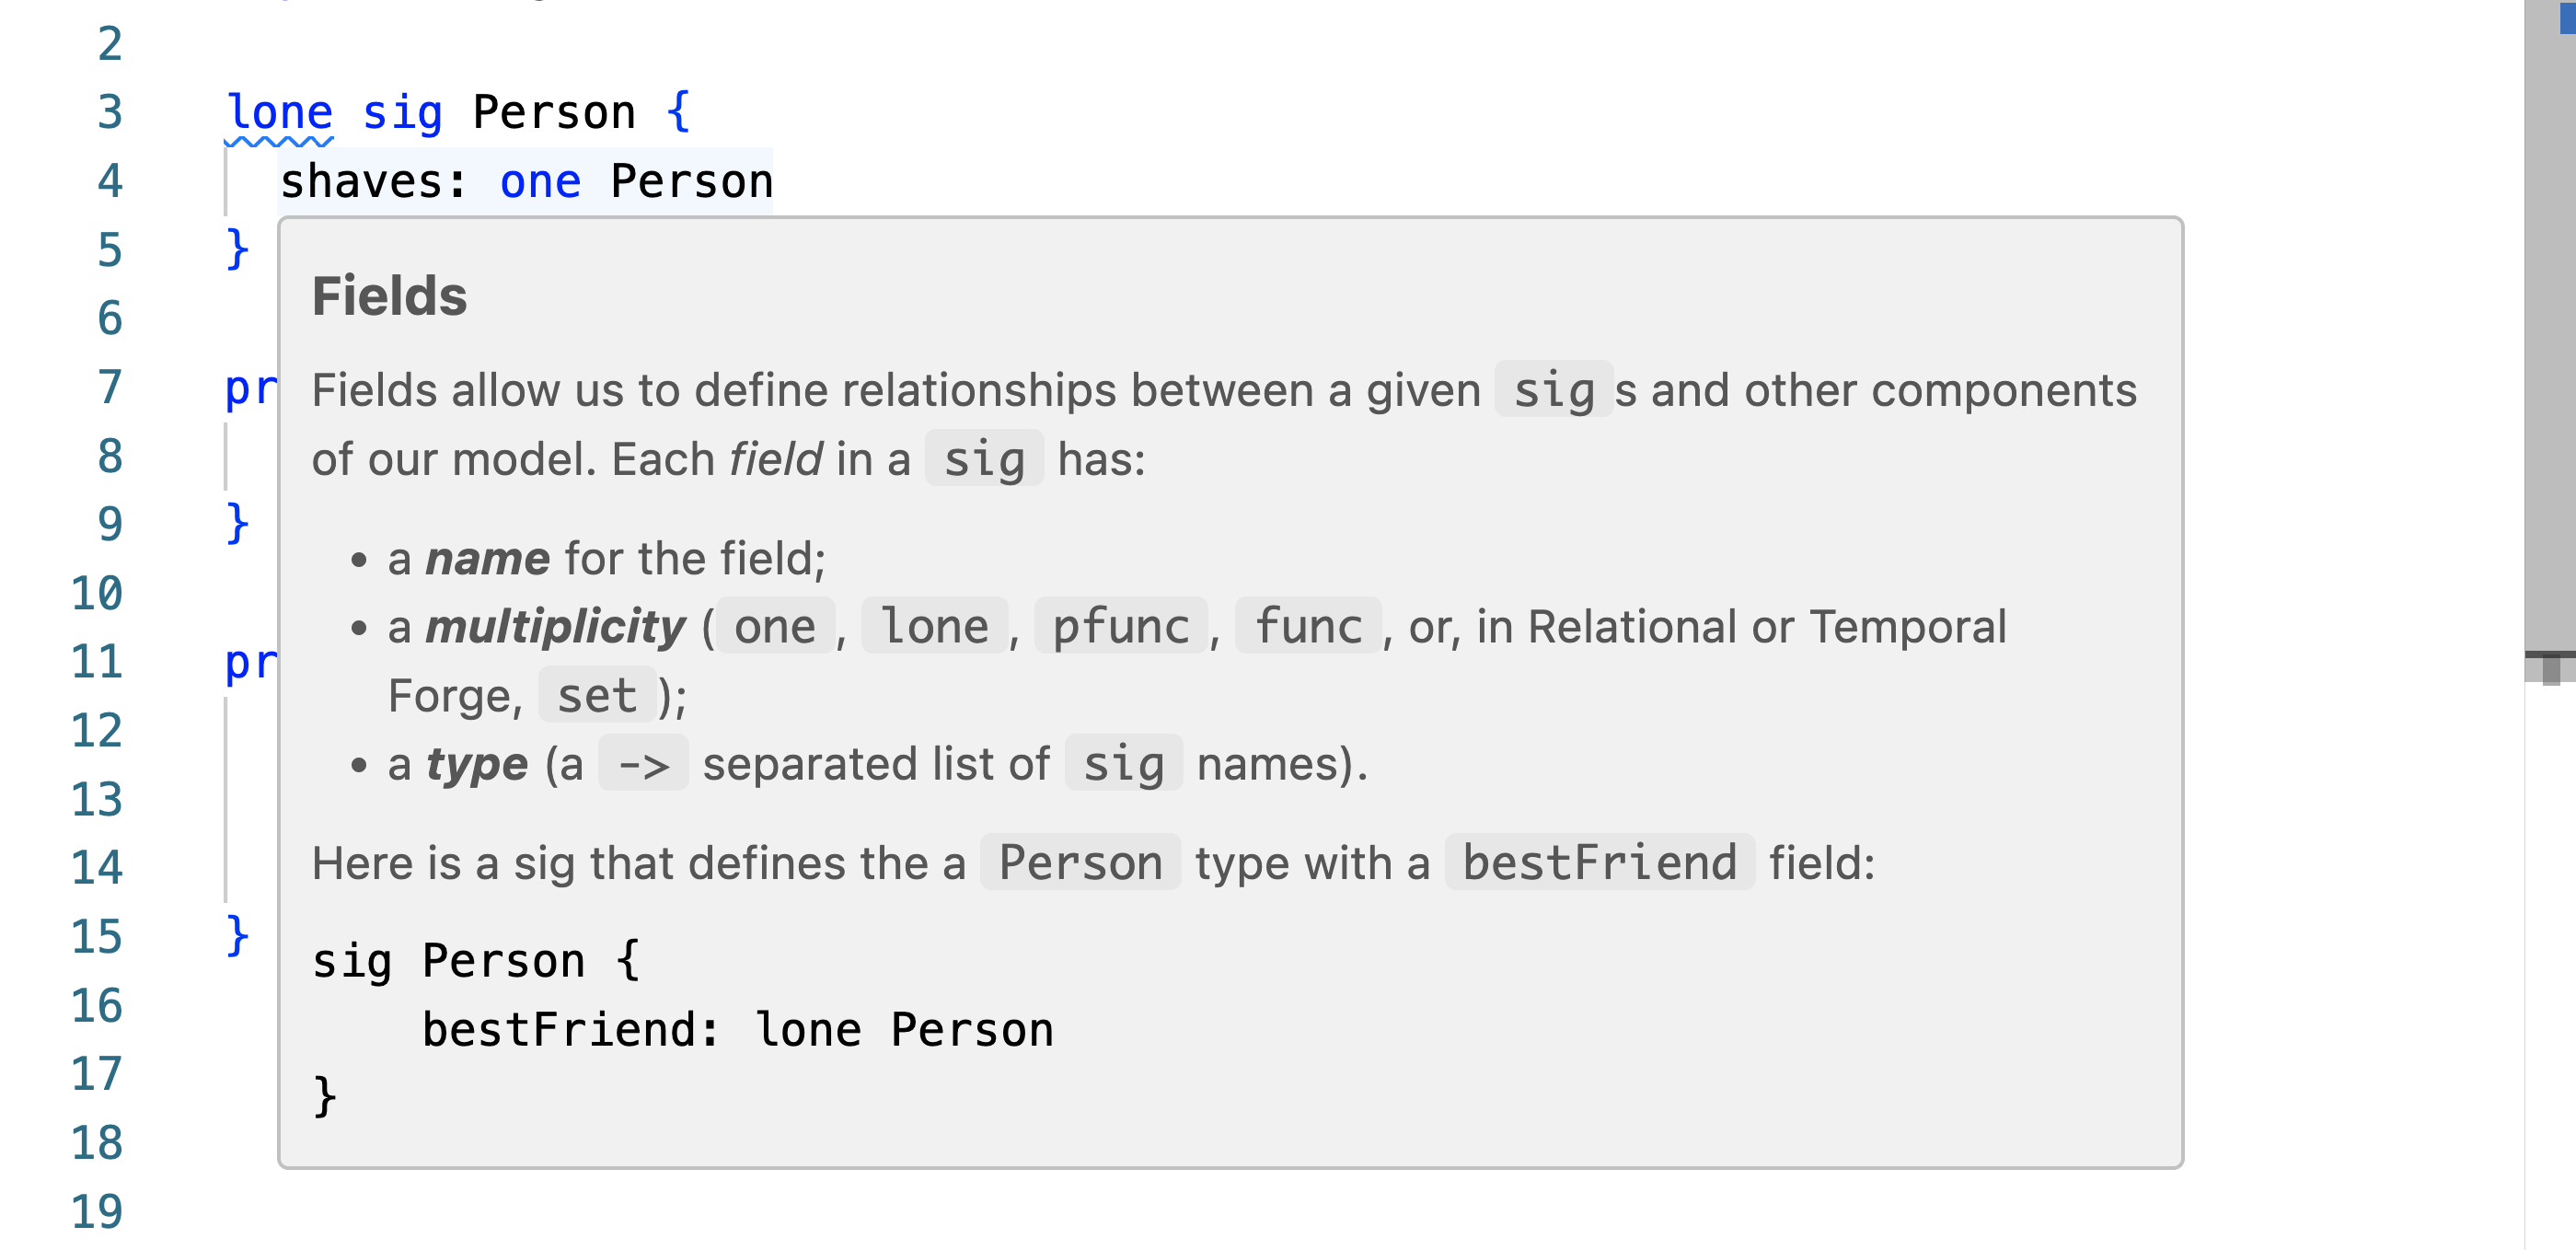
\includegraphics[width=0.6\textwidth,trim={0 0 4cm 0},clip]{images/screenshots/documentation-fields.png}}
  \end{center}
  \caption{We can define our syntax definitions to print with custom documentation text for users new to using Forge syntax. }
  \label{fig:sc-docstrings}
\end{figure}

\begin{figure}
  \centering
  \fbox{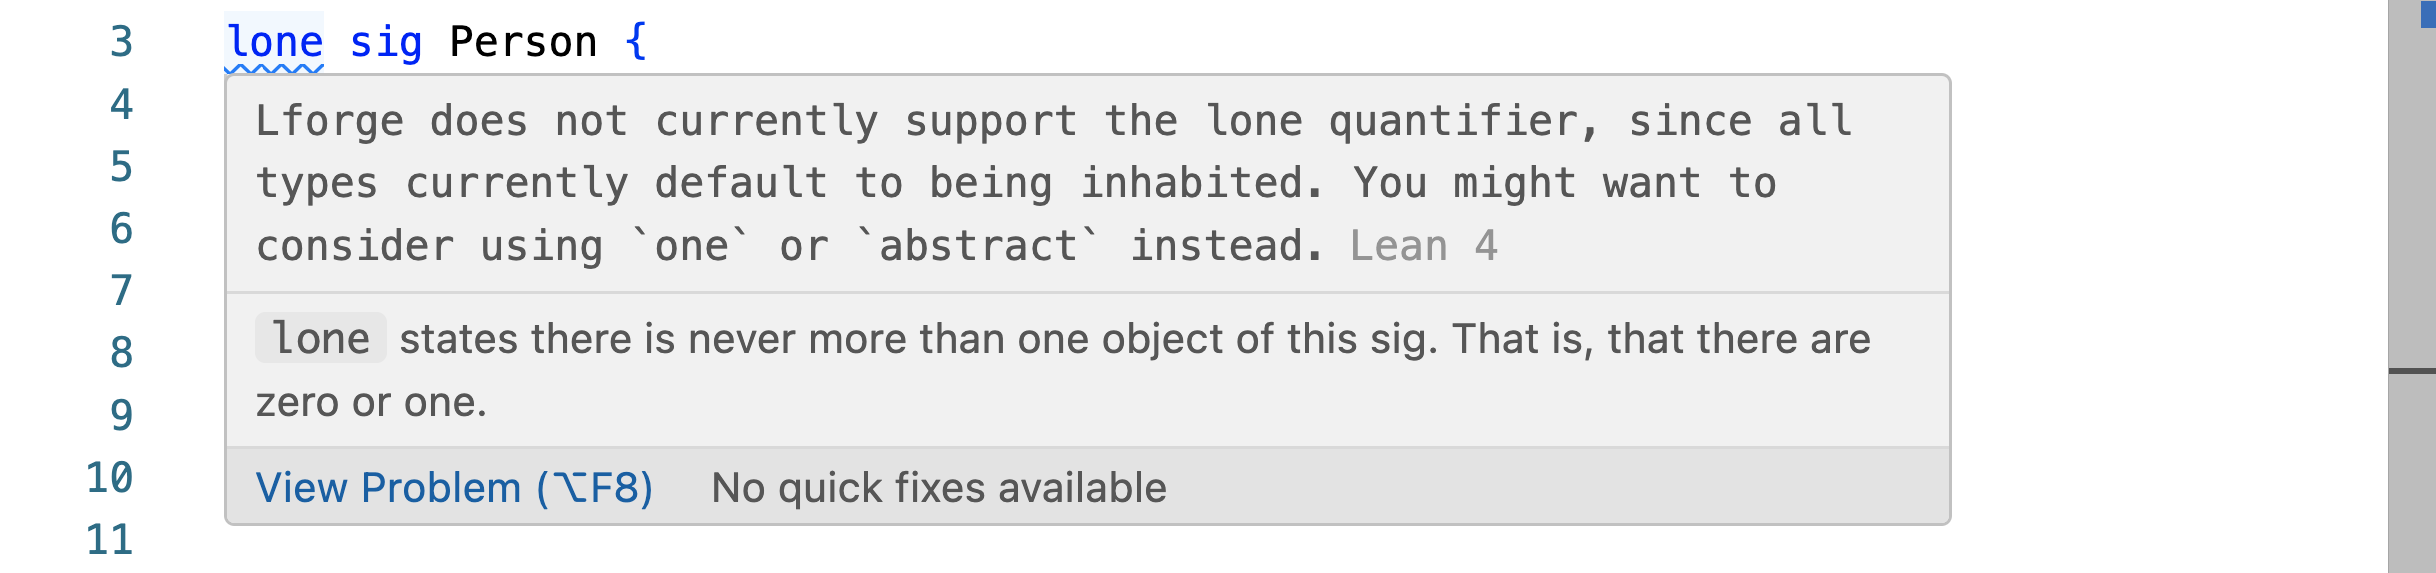
\includegraphics[width=0.6\textwidth,trim={0 0 6cm 0},clip]{images/screenshots/custom-errors.png}}
  \caption{We can define custom error messages with our implementation to prompt users to change their specification if a piece of syntax is ambiguous or not supported.}
  \label{fig:sc-unsupported}
\end{figure}


\subsubsection{Documentation}

As a pedagogical language, Forge has a focus on usability, learnability, and helpful feedback \cite{ngpdbccdlrrvwwk-oopsla-2024}, especially when its parent language Alloy is far more permissive with errors. We follow in the same vein in reporting errors and missing features, and in addition we include documentation on Forge's syntax within Forge's on-hover features. 

Forge documentation is included via docstrings that are inline with our syntax objects (see \cref{sec:parsing}), which is automatically included by Lean's LSP to display on the frontend. \Cref{fig:sc-docstrings} showcases docstrings of varying verbosity for operators as well as declaration syntax. 

Additionally, we need to be clear and verbose about language features that are not supported in \textsc{Lforge}. Since \textsc{Lforge} includes a subset of relational Forge determined by compatibility with Lean's semantics, we prompts users attempting to use unsupported language features with clarification and a request to redefine their statements. \Cref{fig:sc-unsupported} showcases an example of a prompt that \texttt{lone} sig quantifier is unsupported and potentially ambiguous. 

\subsubsection{Error Checking}

Compared to Forge or Racket, Lean (and consequently, \textsc{Lforge}) provides a markedly better experience with error messages and prompting users when there are errors present in their source program. Since Lean runs in the background as a LSP, users immediately get the immediate feedback whether their source code parses and `compiles'.\footnote{Forge translations in Lean are not really executable, so they provide their value in being interactive with the proof system.}

Lean's error locality system allows its error monad to refer to any piece of syntax object to potentially throw an error. This allows us to prompt errors as soon and as granular as possible. \Cref{fig:sc-type-mismatch} illustrates error reporting at the level of specific identifiers. 

\subsubsection{Types}

Lean's dependent type system is both a blessing and a curse when it comes to the task of translating a language with a foreign type system into Lean. While the type system is a highly-optimized algorithm that attempts to resolve type coercions, type classes, and reductions \cite{de2015lean}, it at often delicate and temperamental, especially when we are working at such a low level of emitting Lean \texttt{expr}s, which happens \emph{after} type unification (see \cref{sec:elaboration}). We discuss some of the downsides of such a strict type system in \cref{sec:type-coercions}, and introduced \textsc{Lforge} features that circumvent Lean's restrictions and play into Lean's type system. 

Here, we discuss some of the merits of implementing a DSL designed around Lean's extensive type system. One of the side effects of translating Forge into Lean is that we 

\begin{figure}
  \centering
  \fbox{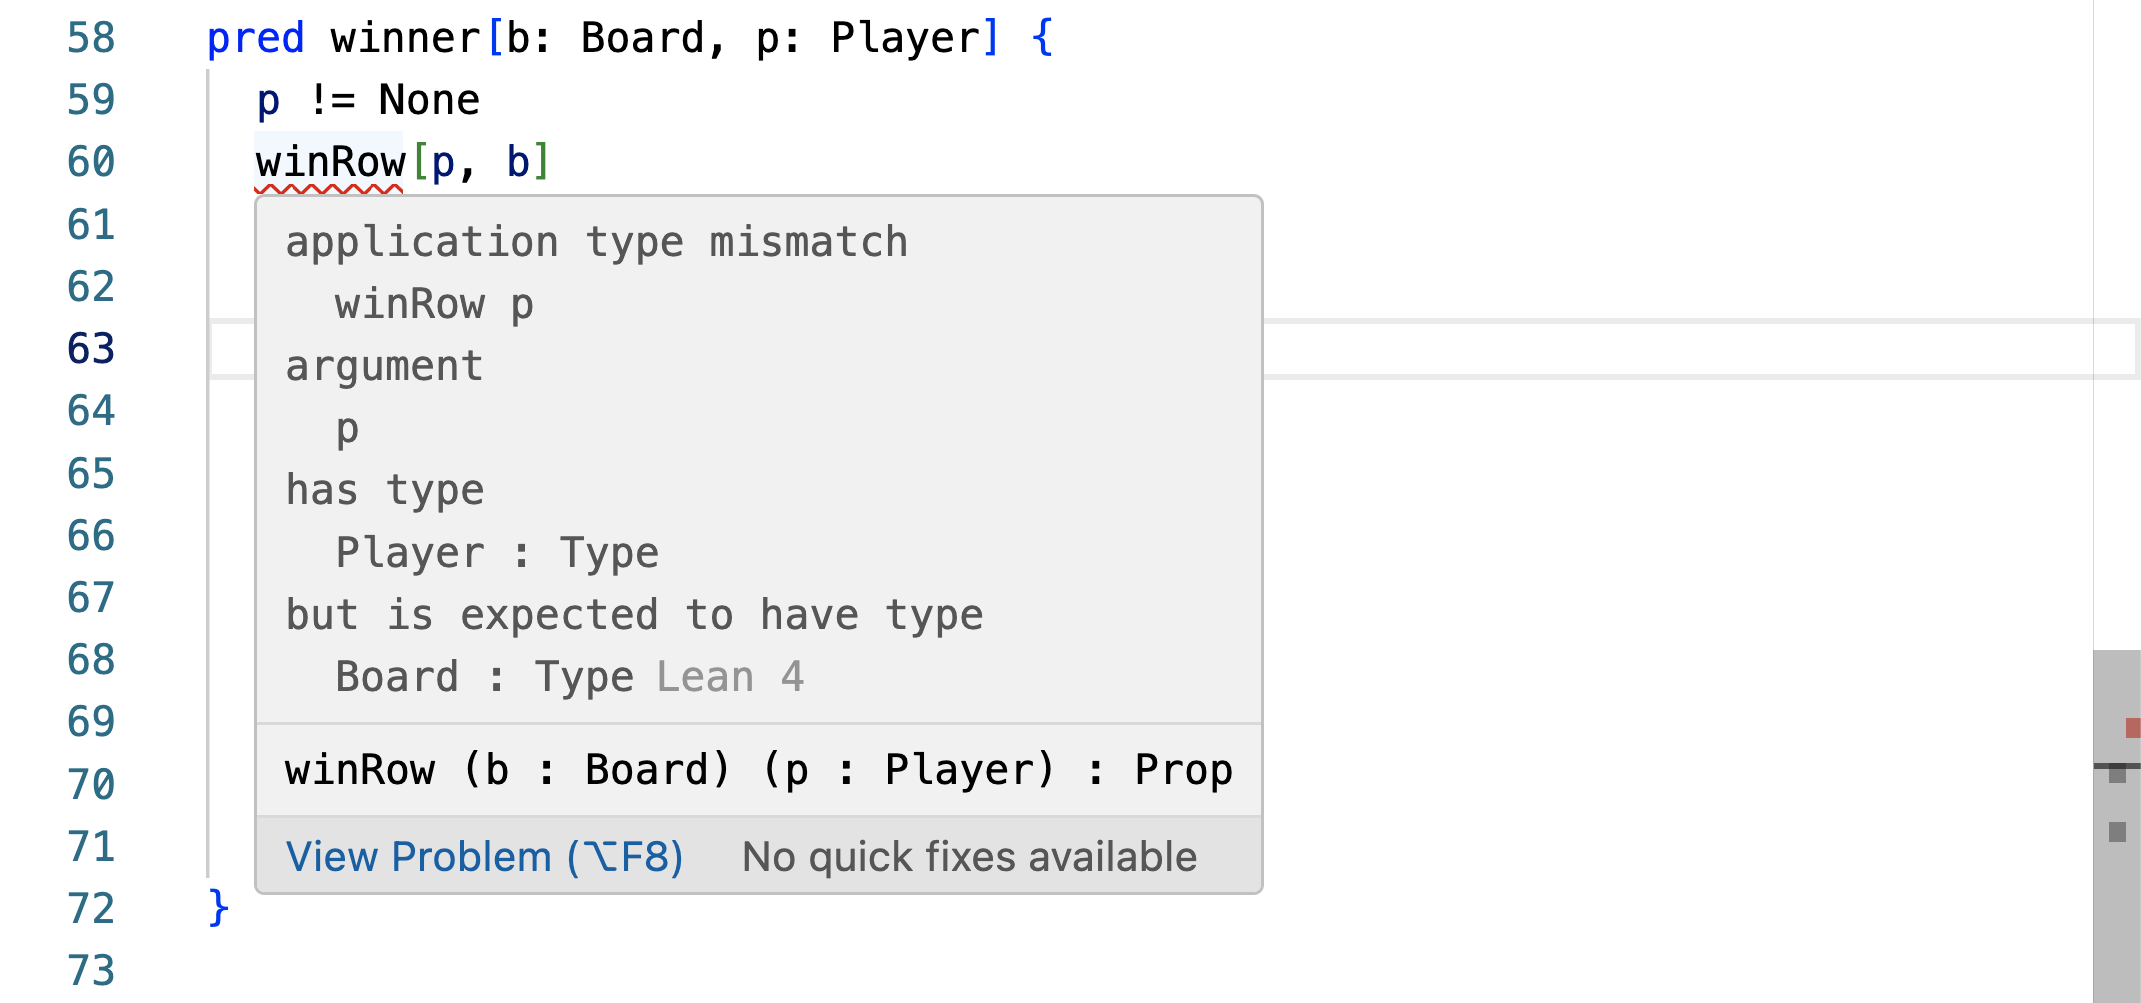
\includegraphics[width=0.6\textwidth,trim={0 0 2cm 0},clip]{images/screenshots/type-check.png}}
  \caption{A Lean error message indicating a type mismatch in our Forge expression.}
  \label{fig:sc-type-mismatch}
\end{figure}

\subsubsection{Mix-ins}

\subsection{A Toy Example, \emph{Continued}}

\subsection{A Realer Example}

\begin{itemize}
  \item Circle back to the earlier example
  \item A more complicated example, potentially with Lean mixins?
\end{itemize}
